\section{Implementation/Development}
The following chapter will cover interesting problems that arose during development, including why they where interesting, how they happened, and how the problem was solved. In addition to this the chapter will also cover the key stages of development and the produced artefacts comparing to that of the user stories/requirements identified above.

\subsection{Encountered issues}
\subsubsection{Room Polygon calculation}
As defined in the design, the rooms will be stored as overlapping rectangles and then later drawn to the screen. The process of calculating the walls and polygon for this was a lot more complicated than initially anticipated. Intensive google searches for this problem returned no results as such a custom algorithm was designed to achieve the goal. Below is the information on the basic overview of how this algorithm works.\\

There's several key steps for generating the polygon, the first of these steps is calculating the walls (excluding entrances) that exist for the given room. This starts out as two separate lists of walls; One for the room and one for all the indents. A function is called to cut-out and merge the two separate lists. The first step is ordering the points of left to right and top to bottom depending on the orientation of the wall. After this has been done the two lists will be looped and checked for overlap, when this occurs several different scenarios of which are listed below.

After this the room walls are adjusted to account for these, this is done by checking for a collision walls and editing the current points of the room wall. There are two conditions that are both applied to wall making three overall cases below are the conditions and what they do, followed by diagram (figure \ref{fig:wallcases}) the resulting three cases.
\begin{itemize}
	\item Indent starts at the same point as the wall (Original wall is removed)
	\item Indent starts after the start point of the wall (Original wall is adjusted to meet the start point)
	\item Indent ends before the end point of the wall (A new wall is added to cover the extra area)
	\item Indent ends at the same point as the wall (No change necessary)	
\end{itemize}
\begin{figure}[h]
	\centering
	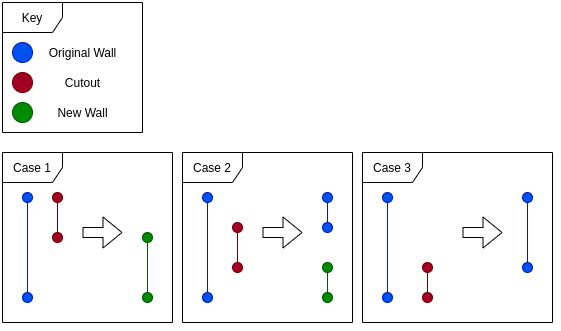
\includegraphics[width=\linewidth]{images/implementation/wallconditions.png}
	\caption{Wall cases}
	\label{fig:wallcases}
\end{figure}

Following the calculation there is one of two paths to follow depending on what's being generated. Given that the walls are being generated the process will be repeated on further cut-outs such as entrances and then returned. If however, the rooms polygon is being calculated the resulting walls will be looped from the wall, the opposite point (walls are pairs of points(A,B)) will then be matched to either point of another wall. The allows the polygon to be calculated all the way round as there should be an even number of walls on each point.

Further work in the future could allow one of many triangulation methods to be used in order to generate a 2D polygon for OpenGL, further expansion could also turn this so that walls are added to the outside as a further polygon so that a 3D projection can be drawn, however both of these are out of scope for the project currently.


\subsubsection{Positioning System/location Calculation}
Location calculation turned out to be a task that couldn't be achieved, the project was ambitious wanting to implement a full indoor mapping system with indoor positioning. Early iterations of the project focused primarily on the infrastructure of the mapping system as opposed to the location calculation in itself, as such it wasn't realised until late into the project the issues that would occur.

The main reason for the failure of this area of the system was possibly because of hardware. The calculated distance measurement was perceived to be sporadic at best with a distance of 1m being calculated as 0cm-200cm. The distance value being calculated on each update would change considerably with large changes being more common (\textgreater 50cm). Due to the lack of a reliable measurement it was established that this wouldn't be applicable in the current state so several options were attempted to solve this. The first option was adding more sensors to see if this would at least render something useable, doing this only highlighted the irregular measurement pattern and further proved this method wasn't reliable.
After these attempts at normalising the data by averaging or throwing out large changes where used both of these methods didn't work either on there own or combined. Doing this also highlighted that deciphering a good measurement from a bad one was difficult without already knowing where the user is which destroys the use of this system, even if this was possible an accurate enough measurement was only obtained in 2 second intervals but normally closer to 4. Time constraints rendered an "IMU sensor fusion" approach as identified in the research by \cite{comer_uwb_vs_ble} non viable which is unfortunate and could be possibly implemented at a later date.

On a positive note the research done did show Bluetooth being a viable option with a range of solutions being developed as a proof of concept such as \cite{kingatua_2020_bluetooth}. For this reason it's believed the cause of these sporadic measurements stems from the hardware used which was a BBC microbit. This could be down to the limitations of the runtime being used, the Bluetooth driver, the antenna of the Bluetooth chip or other reasons. Sadly by the time these conclusions were reached it was too close to the projects deadline to be able to order different hardware such that these theories can be confirmed thus the focus for the remaining portion of the project changed to polishing the rest of the indoor mapping system and android application.

\subsubsubsection{Position classification}
As was identified within the research there are two main ways of relaying someone's location. After the co-ordinate based approach failed the idea of classification was visited and experimented with. This quickly led to positive results and allowed the sporadic measurements from sensors to have some use. The sensors were positioned with one in the centre of each room, doing so meant none or limited direct line of site to another room. Combining this with the extra interference or weakened signal strength that occurs when a signal passes through the wall allowed the system to work mostly accurately with little error. Detection for classification was an algorithm that would identify the sensor with the strongest signal, once this was found, the user's location would be marked at the sensor giving the path to the desired location from there.\\

Further testing was done after on using multiple beacons within a long room to mimic a hallway, doing so would allow a user to see progression through the hallway and therefore allow the navigation system to work effectively. This test also yielded positive results although the level of error was higher. However, it's important to consider the limited space and distance that was available at the test location and spreading the sensor's slightly further apart may have yielded an even better level of classification.\\

Considering the failure of the initial system and then managing a classification system, this is an excellent turn around. Furthering this, although the accuracy isn't a pin point it still allows the user to receive the required information in order to be able to navigate the map in the correct way. The testing of sensors in closer proximity further proved this and a system like this could potentially make a low cost solution for real time mapping application within hospitals, universities and more. This system however would not work for larger open spaces such as museums or conference halls where a greater granular accuracy would be required.

\subsection{Interesting development}
\subsubsection{Rendering engine}
Mostly as a learning exercise a custom pixel based rendering system was written for the rendering of the maps. The writing of this code allowed the learning and research of a range of algorithms for drawing shapes such as: lines, filled polygons, circles and more. All of this gave a great insight and experience into what happens on the back-end of drawing surfaces and canvas APIs within more complicated systems. The way this system was implemented was by using a Screen class which just uses plain Java with it's data being stored in an integer array representing the pixels. This screen class features all the various functions developed for rendering the shapes listed above as well as other useful methods for drawing to the canvas.\\

An unintended advantage for the development of this system was that it separated all the rendering logic from platform specific canvas APIs into it's own API where the only platform specific code is the pushing of this pixel data into a bitmap and finally onto a canvas supplied by Android's canvas API. Having this means it's easier to port the code over to a new system as all of the rendering is now independent of Android's SDK. It's important to remember that this area of the system was implemented as a learning method as such there is no hardware acceleration. However, the frame rate is consistent on an older test device and no issues seem to occur with the level of drawing required.

\subsubsection{Dynamic path nodes \& path finding}
As part of development it was required that a custom point can be added into the path network, so that the path finding algorithm can perform an accurate calculation. A utility class was designed to take the path network and then dynamically link new nodes to that graph. This was achieved by taking the map data and then using a projection it would link to all other nodes, if the projection hits a wall before the path node then a link is not established otherwise a bi-directional link is created to that node. The utility class keeps track of all these dynamic nodes so that only the dynamic nodes can be amended leaving all original data intact. When existing the program of before serialisation of the map the utility is used to destroy all links and the created node. The main interaction of this system is done by the "waypoint" system which stores the user's desired points, the waypoint system returns a path node when called which is fed into the path finding algorithm of which the result is displayed to the user.


